\section{Abstract}
Die strongSwan Open Source VPN Software ist weltweit im Einsatz. Es gibt schon länger die Nachfrage nach einer grafischen Managementoberfläche, welche das Konfigurieren und Starten von VPN Tunnels erleichtert.\\
Zur Umsetzung dieses Problems stellt strongSwan das Versatile IKE Configuration Interface (VICI) zur Verfügung, welches für diverse Programmiersprachen eine JSON-artige Schnittstelle bietet. \\
Im Rahmen dieser Bachelorarbeit ist die Applikation strongMan entstanden, die auf dem Python Webframework Django basiert und seine Daten in einer eigenen Datenbank persistiert.\\

Die kurze Installation, welche optional auch einen systemd Service beinhaltet. Nach dem Userlogin kann über das Webinterface verschiedene IPsec Verbindungen konfiguriert werden. Der Benutzer kann zwischen mehreren vordefinierten IKEv2 Authentisierungsmethoden auswählen und dann mithilfe eines benutzerfreundlichen Formulars den Tunnel in zwei Schritten konfigurieren. 

Wird eine Verbindung auf der Hauptübersicht gestartet, wandelt strongMan die Konfiguration in ein Dictionary um und übergibt es mit den entsprechenden Daten dem VICI Interface. Sobald die Verbindung steht, stehen Informationen über Traffic Selectoren und Dateninput und Output zur Verfügung.

Auf der About Seite sind weitere Informationen über strongSwan und seine installierten Plugins aufgelistet.\\

\begin{wrapfigure}{r}{0.5\textwidth}
  \begin{center}
    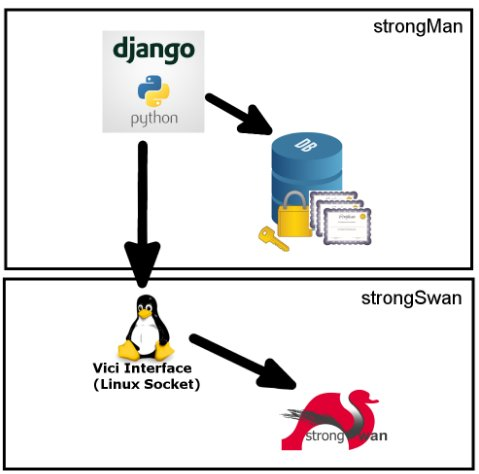
\includegraphics[width=230px]{images/abstract_overview.jpg}
  \end{center}
    \caption[Übersicht]{Übersicht}
\end{wrapfigure}

Eine interne Zertifikatsverwaltung managt die Zertifikate und die privaten Schlüssel, welche von den Verbindungen gebraucht werden. Wichtige Felder wie der CName können direkt in der Zertifikatsvorschau eingesehen werden.\\

Dieses Projekt legte einen starken Fokus auf die Usability der einzelne Ansichten und Formulare, was in einer überlegten Bedienbarkeit auch für unerfahrene Benutzer resultierte.\\

Die Applikation strongMan deckt zur Zeit nur Client Funktionalitäten ab. In einem nächsten Schritt ist es möglich die Anwendung so zu erweitern, dass auch Serverfunktionalitäten und somit IPsec Server konfiguriert werden können. Dies erfordert die weitere Implementierung von möglichen Konfigurationen für den Server, eine Oberflächenüberarbeitung zur Darstellung von einer grösseren Anzahl von Verbindungen/Zertifikaten, das Management von Child SA's und weitere Statistikinformationen.